
\section{Netzgerät}
\label{section:netzgeraet_1}
\begin{frame}%STARTCONTENT

\begin{columns}
    \begin{column}{0.48\textwidth}
    \begin{itemize}
  \item Netzgerät wandelt Wechselspannung von 230 V aus der Steckdose in kleinere Gleichspannung um
  \item Im Amateurfunk wird häufig 13,8 V für Transceiver verwendet
  \end{itemize}

    \end{column}
   \begin{column}{0.48\textwidth}
       
\begin{figure}
    \DARCimage{0.85\linewidth}{740include}
    \caption{\scriptsize Netzgerät}
    \label{n_netzgeraet}
\end{figure}


   \end{column}
\end{columns}

\end{frame}

\begin{frame}
\only<1>{
\begin{QQuestion}{ND101}{Ein Mobilfunktransceiver ist an ein Netzgerät angeschlossen. Welche Aufgabe hat das Netzgerät?}{Die Stabilisierung der \qty{230}{\V} Wechselspannung.}
{Erzeugung einer Wechselspannung aus einer Gleichspannung.}
{Erzeugung einer Gleichspannung aus dem \qty{230}{\V} Wechselspannungsnetz.}
{Eine Internetverbindung zum Funkgerät herzustellen.}
\end{QQuestion}

}
\only<2>{
\begin{QQuestion}{ND101}{Ein Mobilfunktransceiver ist an ein Netzgerät angeschlossen. Welche Aufgabe hat das Netzgerät?}{Die Stabilisierung der \qty{230}{\V} Wechselspannung.}
{Erzeugung einer Wechselspannung aus einer Gleichspannung.}
{\textbf{\textcolor{DARCgreen}{Erzeugung einer Gleichspannung aus dem \qty{230}{\V} Wechselspannungsnetz.}}}
{Eine Internetverbindung zum Funkgerät herzustellen.}
\end{QQuestion}

}
\end{frame}

\begin{frame}
\only<1>{
\begin{QQuestion}{ND102}{Welche Spannung liefert ein Netzgerät für einen Mobilfunk-Transceiver üblicherweise?}{ca. \qty{13,8}{\V} Gleichspannung}
{ca. \qty{230}{\V} Gleichspannung}
{ca. \qty{13,8}{\V} Wechselspannung}
{ca. \qty{230}{\V} Wechselspannung}
\end{QQuestion}

}
\only<2>{
\begin{QQuestion}{ND102}{Welche Spannung liefert ein Netzgerät für einen Mobilfunk-Transceiver üblicherweise?}{\textbf{\textcolor{DARCgreen}{ca. \qty{13,8}{\V} Gleichspannung}}}
{ca. \qty{230}{\V} Gleichspannung}
{ca. \qty{13,8}{\V} Wechselspannung}
{ca. \qty{230}{\V} Wechselspannung}
\end{QQuestion}

}
\end{frame}

\begin{frame}
\frametitle{Schutzkontakt}
\begin{columns}
    \begin{column}{0.48\textwidth}
    \begin{itemize}
  \item Beim \emph{Schutzkontaktstecker} gibt es drei Pole
  \item L- und N-Leiter durch Stifte
  \item Dort liegt die 230 V-Spanung an
  \item \emph{Schutzkontakt} ist der dritte Pol
  \item PE-Leiter durch äußere Schleifkontakte
  \end{itemize}

    \end{column}
   \begin{column}{0.48\textwidth}
       
\begin{figure}
    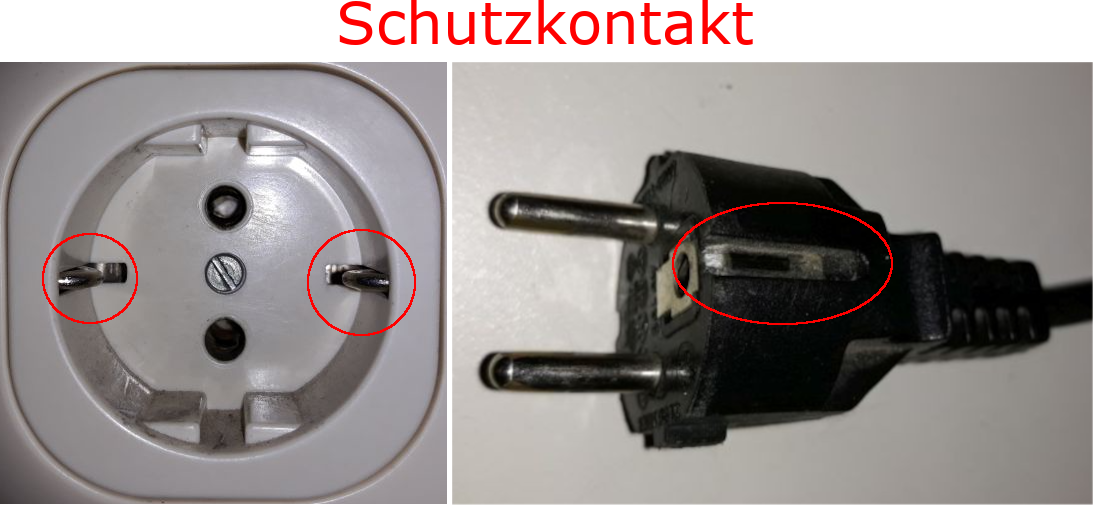
\includegraphics[width=0.85\textwidth]{foto/86}
    \caption{\scriptsize Schutzkontakt an einer Steckdose und Schukostecker}
    \label{n_schutzkontakt}
\end{figure}

   \end{column}
\end{columns}

\end{frame}

\begin{frame}
\only<1>{
\begin{QQuestion}{ND109}{Welche Verbindung stellt der Schutzkontakt in einem Schutzkontakt-Stecker (Schuko-Stecker) her?}{Verbindung zum L-Leiter der Steckdose}
{Verbindung zwischen PE- und N-Leiter in der Steckdose}
{Verbindung zum N-Leiter der Steckdose}
{Verbindung zum PE-Leiter der Steckdose}
\end{QQuestion}

}
\only<2>{
\begin{QQuestion}{ND109}{Welche Verbindung stellt der Schutzkontakt in einem Schutzkontakt-Stecker (Schuko-Stecker) her?}{Verbindung zum L-Leiter der Steckdose}
{Verbindung zwischen PE- und N-Leiter in der Steckdose}
{Verbindung zum N-Leiter der Steckdose}
{\textbf{\textcolor{DARCgreen}{Verbindung zum PE-Leiter der Steckdose}}}
\end{QQuestion}

}
\end{frame}

\begin{frame}
\frametitle{Gleichspannungsausgang}

\begin{figure}
    \DARCimage{0.85\linewidth}{680include}
    \caption{\scriptsize Anschluss von Netzgerät und TRX}
    \label{n_Netzgeraet_TRX}
\end{figure}
\begin{columns}
    \begin{column}{0.48\textwidth}
    \begin{itemize}
  \item Ist zweipolig zum Transceiver
  \item Klemmen sind in der Regel farbig
  \end{itemize}

    \end{column}
   \begin{column}{0.48\textwidth}
       
    \pause
    \begin{itemize}
  \item Rot für Plus
  \item Schwarz für Minus
  \item Polung beachten!
  \end{itemize}



   \end{column}
\end{columns}

\end{frame}

\begin{frame}
\only<1>{
\begin{QQuestion}{ND104}{Warum ist die Spannungsversorgungsleitung vom externen Netzteil zum Transceiver zweipolig ausgeführt?}{Damit die Spannungsreduzierung nicht zu hoch wird.}
{Damit von beiden Polen des Netzteils der Strom zum Transceiver fließen kann.}
{Der Transceiver nutzt eine Leitung, die andere Leitung dient zur Erdung.
}
{Damit der Stromkreis über den Transceiver geschlossen werden kann.}
\end{QQuestion}

}
\only<2>{
\begin{QQuestion}{ND104}{Warum ist die Spannungsversorgungsleitung vom externen Netzteil zum Transceiver zweipolig ausgeführt?}{Damit die Spannungsreduzierung nicht zu hoch wird.}
{Damit von beiden Polen des Netzteils der Strom zum Transceiver fließen kann.}
{Der Transceiver nutzt eine Leitung, die andere Leitung dient zur Erdung.
}
{\textbf{\textcolor{DARCgreen}{Damit der Stromkreis über den Transceiver geschlossen werden kann.}}}
\end{QQuestion}

}
\end{frame}

\begin{frame}
\only<1>{
\begin{QQuestion}{ND103}{Warum ist die Spannungsversorgungsleitung vom Gleichspannungsnetzteil zum Transceiver zweipolig ausgeführt?}{Der Strom fließt in beide Leiter hinein und über die Erde zum Netzteil zurück.}
{Der Strom fließt in einem Leiter hin und im anderen Leiter wieder zurück.}
{Damit insgesamt mehr Strom fließen kann.}
{Der Strom fließt aus beiden Leitern heraus und über die Erde zum Netzteil zurück.}
\end{QQuestion}

}
\only<2>{
\begin{QQuestion}{ND103}{Warum ist die Spannungsversorgungsleitung vom Gleichspannungsnetzteil zum Transceiver zweipolig ausgeführt?}{Der Strom fließt in beide Leiter hinein und über die Erde zum Netzteil zurück.}
{\textbf{\textcolor{DARCgreen}{Der Strom fließt in einem Leiter hin und im anderen Leiter wieder zurück.}}}
{Damit insgesamt mehr Strom fließen kann.}
{Der Strom fließt aus beiden Leitern heraus und über die Erde zum Netzteil zurück.}
\end{QQuestion}

}
\end{frame}

\begin{frame}
\only<1>{
\begin{QQuestion}{ND105}{Wie sind die Klemmen einer \qty{13,8}{\V} Gleichspannungsversorgung gekennzeichnet?}{Pluspol schwarz, Minuspol grüngelb}
{Pluspol blau, Minuspol rot}
{Pluspol rot, Minuspol schwarz}
{Pluspol braun, Minuspol grüngelb}
\end{QQuestion}

}
\only<2>{
\begin{QQuestion}{ND105}{Wie sind die Klemmen einer \qty{13,8}{\V} Gleichspannungsversorgung gekennzeichnet?}{Pluspol schwarz, Minuspol grüngelb}
{Pluspol blau, Minuspol rot}
{\textbf{\textcolor{DARCgreen}{Pluspol rot, Minuspol schwarz}}}
{Pluspol braun, Minuspol grüngelb}
\end{QQuestion}

}
\end{frame}

\begin{frame}
\only<1>{
\begin{QQuestion}{ND106}{Worauf ist beim Anschluss eines Gleichspannungsnetzteils an einen Transceiver  besonders zu achten?}{Korrekte Verbindung zur Antenne}
{Richtige Polung des Schutzkontaktsteckers}
{Polungsrichtiger Anschluss der Stromversorgungsleitung zum Transceiver}
{Polungsrichtiger Anschluss des SWR-Meters}
\end{QQuestion}

}
\only<2>{
\begin{QQuestion}{ND106}{Worauf ist beim Anschluss eines Gleichspannungsnetzteils an einen Transceiver  besonders zu achten?}{Korrekte Verbindung zur Antenne}
{Richtige Polung des Schutzkontaktsteckers}
{\textbf{\textcolor{DARCgreen}{Polungsrichtiger Anschluss der Stromversorgungsleitung zum Transceiver}}}
{Polungsrichtiger Anschluss des SWR-Meters}
\end{QQuestion}

}
\end{frame}

\begin{frame}
\only<1>{
\begin{QQuestion}{ND107}{Welche Folge kann eine Verpolung der Leitung vom Netzteil zum Transceiver nach sich ziehen?}{Ausfall der Backup-Batterie im Transceiver}
{Verzerrung des Sendesignals}
{Beschädigung des Funkgeräts}
{Verzerrung des Empfangssignals}
\end{QQuestion}

}
\only<2>{
\begin{QQuestion}{ND107}{Welche Folge kann eine Verpolung der Leitung vom Netzteil zum Transceiver nach sich ziehen?}{Ausfall der Backup-Batterie im Transceiver}
{Verzerrung des Sendesignals}
{\textbf{\textcolor{DARCgreen}{Beschädigung des Funkgeräts}}}
{Verzerrung des Empfangssignals}
\end{QQuestion}

}
\end{frame}

\begin{frame}
\frametitle{Feinsicherungen}
\begin{columns}
    \begin{column}{0.48\textwidth}
    
\begin{figure}
    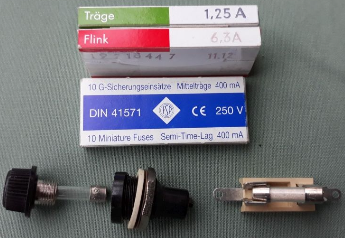
\includegraphics[width=0.85\textwidth]{foto/88}
    \caption{\scriptsize Feinsicherungen}
    \label{n_feinsicherungen}
\end{figure}

    \end{column}
   \begin{column}{0.48\textwidth}
       \begin{itemize}
  \item Unterbrechen Stromfluss im Fehlerfall (Kurzschluss oder Überlastung)
  \item Schmelzsicherungen in denen ein dünner Draht schmilzt
  \item \emph{Durchgebrannte Sicherung} bzw. \emph{thermische Abschaltung}
  \end{itemize}

   \end{column}
\end{columns}

\end{frame}

\begin{frame}
\frametitle{Feinsicherungen austauschen}
\begin{itemize}
  \item Erst die Ursache beheben
  \item Durch gleichartige ersetzen
  \item Stromstärke und Auslösecharakteristik
  \end{itemize}
\end{frame}

\begin{frame}
\frametitle{Kenngrößen von Feinsicherungen}
\begin{table}
\begin{DARCtabular}{ccc}
     Auslösecharakteristik  & Kennzeichen  & Abschaltzeit bei zehnfachem Nennstrom   \\
     flink  & F  & max. 30 ms  \\
     mittelträge  & MT  & max. 90 ms   \\
     träge  & T  & max. 300 ms   \\
\end{DARCtabular}
\caption{Kenngrößen von Feinsicherungen}
\label{n_feinsicherung}
\end{table}
\end{frame}

\begin{frame}
\frametitle{Elektronische Begrenzung}
\begin{itemize}
  \item In hochwertigen Netzgeräten
  \item Im Kurzschlussfall wird die Stromstärke begrenzt
  \item \emph{Kurzschlussstrombegrenzung}
  \item Kein Austausch von Sicherungen notwendig
  \end{itemize}
\end{frame}%ENDCONTENT
